\textbf{Пример 1}

\texttt{take\_photos(5, 7, 2, [0, 4, 4, 4, 4], [3, 4, 6, 5, 6])}

В этом примере есть сетка $7 \times 7$ с $5$ интересными точками. Интересные точки расположены в 4 различных клетках: $(0, 3)$, $(4, 4)$, $(4, 5)$ и $(4, 6)$. Можно сделать не более $2$ фотографий в хорошем качестве.

Например, один вариант сфотографировать все интересные точки двумя фотографиями: сделать одну фотографию в форме квадрата $6 \times 6$ с противоположными углами $(0, 0)$ и $(5, 5)$, и вторую $3 \times 3$ с противоположными углами $(4, 4)$ и $(6, 6)$. Если спутник сделает эти две фотографии, спутнику будет необходимо послать фотографии в хорошем качестве для $41$ клетки. Это количество не оптимально.

Оптимальное решение~--- сделать одну из фотографий в форме квадрата $4 \times 4$ с противоположными углами $(0, 0)$ и $(3, 3)$ и другую фотографию в форме квадрата $3 \times 3$ с противоположными углами $(4, 4)$ и $(6, 6)$. Для этого потребуется послать только $25$ фотографий клеток, что является оптимальным, поэтому \texttt{take\_photos} должна вернуть $25$.

Обратите внимание, что достаточно сфотографировать клетку $(4, 6)$ один раз, несмотря на то, что она содержит две интересных точки.

Этот пример показан на рисунке ниже. Самый левый рисунок показывает сетку, соответствующую примеру. Средняя картинка показывает не оптимальное решение, в котором сфотографирована $41$ клетка. На самой правой картинке показано оптимальное решение.

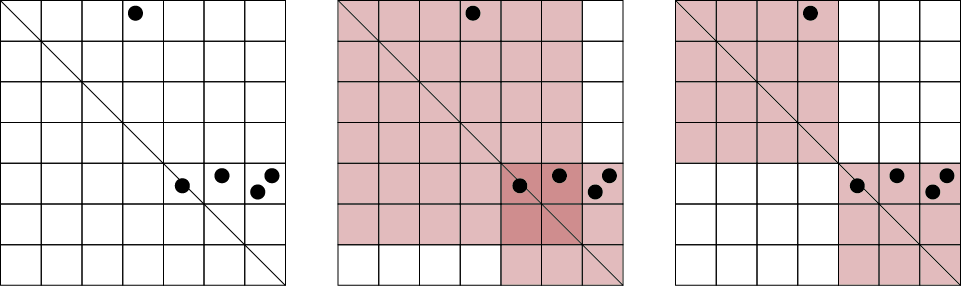
\includegraphics[scale=1.5]{example1.png}

\textbf{Пример 2}

\texttt{take\_photos(2, 6, 2, [1, 4], [4, 1])}

В этом примере есть $2$ интересных точки расположенных симметрично: в клетках $(1, 4)$ и $(4, 1)$. Любая фотография, содержащая одну из этих точек, содержит и другую. Таким образом, достаточно сделать одну фотографию.

На рисунке ниже изображен пример и его оптимальное решение. В этом решении спутник делает одну фотографию, на которую попадает $16$ клеток.

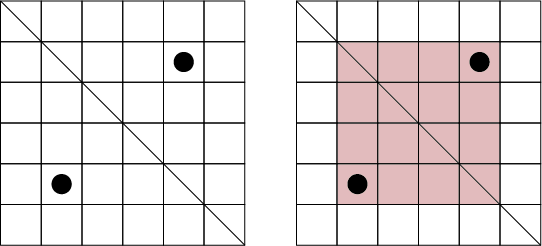
\includegraphics[scale=1.5]{example2.png}